\section{Ontology}
\label{sec:ontology}

% Explain what an ontology is and refer to summary of this paper
According to Gruber \cite{gruber1993ontology}, an ontology is an ``explicit specification of a conceptualization''. As such, in this paper, several concepts are specified and its relations are further detailed. A summary of the ontology is presented in Table~\ref{tab:ontology}.

\begin{table}
	\begin{center}
		\caption{Summary of the ontology presented in this paper.}
		\label{tab:ontology}
		\begin{tabularx}{\linewidth}{p{3em} X X}
			\toprule
			Term & Characteristics & ``has'' \\ \otoprule
			Scenario class & Qualitative description of scenario & Scenarios \newline Other (less generic) scenario classes \newline One or multiple tags \\
			Scenario & Quantitative description \newline Time interval & One or multiple events \newline One or multiple activities \newline Ego vehicle \newline Static environment \newline Dynamic environment \\
			Event & Time instant \newline Mode transition (i.e. change of input, parameter or state) & \\
			Activity & Inter-event time interval \newline Quantitative description of (changing) state & Model that describes the way the state evolves \\
			\bottomrule
		\end{tabularx}
	\end{center}
\end{table}

% Explain section
First, the context for which this paper describes the ontology is described in Section~\ref{sec:context}. In Section~\ref{sec:scenario definition}, a definition of the term \emph{scenario} is given. Next, a discussion on the scenario classes is provided. As presented in Section~\ref{sec:scenario definition}, a scenario consists of events. The definition of an event is presented in Section~\ref{sec:events}.

\subsection{Context of a scenario}
\label{sec:context}

% Scenario definitions are very diverse --> context is important
Because the notion of scenario is used in many different contexts, a high diversity in definitions of this notion exists (for an overview, see \cite{vannotten2003updated, bishop2007scentechniques}). Therefore, it is reasonable to assume that ``there is no `correct' scenario definition'' \cite{vannotten2003updated}. As a result, to define the notion of scenario, it is important to consider the context in which it will be used.

% Explain context
% - Scenarios can be defined by human expert (knowledge driven) or by using data (Stellet et al.)
% - Could be used for assessment (Adaptive paper, pegasus, stellet et al., )
In this paper, the context of a scenario is the assessment of automated vehicles. It is assumed that the assessment methodology uses scenarios (i.e., test cases) for which some resulting metrics are compared with a reference \cite{stellet2015taxonomy}. 
% - Scenarios that an (automated) vehicle can encounter
The ultimate goal is to build a database with all relevant scenarios that an AV has to cope with when driving in the real world \cite{putz2017pegasus}. Hence, a scenario should be a description of a potential use case of an automated vehicle. 
% Whether these scenarios are obtained with a knowledge-based approach \cite{gietelink2004systemvalidation, stellet2015taxonomy} or with a data-driven approach \cite{deGelder2017assessment, stellet2015taxonomy}, a clear and unambiguous definition of such a test scenario is required. 

In this paper, \emph{scenario} can refer to either an observed scenario in (real-world driving) data, i.e., a real-world scenario, or a scenario that is used for testing AVs, i.e., a test case. Note that, typically, the difference between the two is that with a real-world scenario, the activity of all actors is described, while for a test case, some goals are specified for the system under test (e.g., the goal could be to drive from A to B) instead of its activity. 

%In the case of a data-driven approach, the test scenarios are generated through analysis of observed scenarios in (real-life driving) data. Because the observed scenarios can roughly be described in a similar manner as the test scenarios, we will refer to these observed and test scenarios as scenarios.

\subsection{Definition of scenario}
\label{sec:scenario definition}

%Van Notten et al.\ \cite{vannotten2003updated} present an overview of the diversity in the scenarios. Van Notten et al.\ state that ``in view of the observed variety in scenario approaches'', it is assumed ``that there is no `correct' scenario definition or approach. However, the typology uses the following broad working definition: scenarios are descriptions of possible futures that reflect different perspectives on the past, the present and the future.''

% Techniques for scenario development
%Where the contribution of Van Notten et al.\ \cite{vannotten2003updated} relate more to the overall scenario project, Bishop et al.\ \cite{bishop2007scentechniques} focus more on the techniques to produce scenarios, i.e.\ the process of creating scenarios. These scenario development techniques vary from genius forecasting \cite{kahn1962}, event sequences with probability trees \cite{covaliu1995representation} and sensitivity analysis \cite{saltelli2008global}.

% How to apply to real-world traffic scenarios
%If it was not clear yet, the contributions of Van Notten et al.\ \cite{vannotten2003updated} and Bishop et al.\ \cite{bishop2007scentechniques} point out that the notion of scenario is very broad. We are interested in scenarios that can be used in the context of road traffic, which limits the scope of what a scenario is. The description of a scenario by Go and Carroll \cite{go2004blind} is more suited to our needs.
% Definition according to Go and Carroll
Go~and~Carroll~\cite{go2004blind} describe a scenario within the field of system design. They define a scenario as ``a description that contains (1) actors, (2) background information on the actors and assumptions about their environment, (3) actors' goals or objectives, and (4) sequences of actions and events. Some applications may omit one of the elements or they may simply or implicitly express it. Although, in general, the elements of scenarios are the same in any field, the use of scenarios is quite different.'' 

% Definition according to Geyer et al.
Geyer~et~al.~\cite{geyer2014} describe a scenario within the context of automated driving. They use the metaphor of a movie or a storybook for describing a scenario. Geyer~et~al.\ state that ``a scenario includes at least one situation within a scene including the scenery and dynamic elements. However, [a] scenario further includes the ongoing activity of one or both actors.'' For a further explanation of the terms situation, scene, and scenery, see \cite{geyer2014}. It is mentioned that the action of the driver and/or automation might be predefined. In \cite{geyer2014}, the meaning of action is not detailed.
%In an example of a so-called crossway scenario, they mention that the course of events might be different. For example, when a car keeps constant speed and then turns right, the scenario consists of one situation. The car might also first decelerate, accelerate and decelerate before turning right. In this case, the scenario consists of four situations.

% Definition according to Ulbrich et al.
Ulbrich~et~al.~\cite{ulbrich2015} also define a scenario in the context of automated driving. They define a scenario as ``the temporal development between several scenes in a sequence of scenes. Every scenario starts with an initial scene. Actions \& events as well as goals \& values may be specified to characterize this temporal development in a scenario. Other than a scene, a scenario spans a certain amount of time.'' They state that actions and events link the different scenes. A further description of actions and events is not given in \cite{ulbrich2015}.

% Definition according to Elrofai et al.
Another definition of a scenario in the context of automated driving is given by Elrofai~et~al.~\cite{elrofai2016scenario}. They define scenario as ``the combination of actions and maneuvers of the host vehicle in the passive [i.e., static] environment, and the ongoing activities and maneuvers of the immediate surrounding active [i.e., dynamic] environment for a certain period of time.'' They further mention that the duration of a scenario typically is in the order of seconds.

% "Requirements"
Before providing the definition of the notion of scenario, the characteristics of this notion are listed.

% Order of seconds
\subsubsection{A scenario corresponds to a time interval}
The aforementioned definitions \cite{go2004blind, geyer2014, ulbrich2015, elrofai2016scenario} state that a scenario corresponds to a time interval. Van Notten~et~al.~\cite{vannotten2003updated} call such a scenario a chain scenario (``like movies''), as opposed to a snapshot scenario, i.e., a scenario that describes the state at a time instant (``like photos''). The duration of a scenario is in the order of seconds, as explicitly mentioned by Elrofai~et~al.~\cite{elrofai2016scenario}. Though the duration is not mentioned by Ulbrich~et~al.~\cite{ulbrich2015}, the presented example is in the order of seconds. Furthermore, other scenarios regarding (automated) driving are also in the order of seconds, e.g., see \cite{gietelink2006development, zofka2015datadrivetrafficscenarios, roesener2017comprehensive, karaduman2013interactivebehavior, hulshof2013autonomous, englund2016grand}.

% Scenarios consists of one or several events
\subsubsection{A scenario consists of one or several events \cite{vannotten2003updated, go2004blind, geyer2014, ulbrich2015, kahn1962, englund2016grand, schoemaker1993multiple, cuppens2002alert, bach2016modelbased}}
It can be helpful to develop scenarios using events \cite{bishop2007scentechniques}. Thus, a scenario could be defined as a particular sequence of events or, as Kahn \cite{kahn1962} writes, ``a scenario results from an attempt to describe in more or less detail some hypothetical sequence of events''. Furthermore, Geyer~et~al.~\cite{geyer2014} and Ulbrich~et~al.~\cite{ulbrich2015} use the notion of event for describing a scenario, although they do not provide a definition of the term \emph{event}. In \cref{sec:events}, we will elaborate on the notion of \emph{event}.

% Semantically described
\subsubsection{Real-world traffic scenarios are quantitative scenarios}
Regarding the nature of the data, a scenario can be either qualitative or quantitative \cite{vannotten2003updated}. Real-life traffic scenarios are quantitative scenarios, such that they are, e.g., suitable for simulation purposes. A scenario, however, can be described qualitatively, such that it is readable and understandable for human experts. Providing a qualitative description of a quantitative scenario has become known as a story-and-simulation approach \cite{alcamo2001scenarios}. Note that several quantitative scenarios might have the same qualitative description; thus a qualitative description of a scenario does not uniquely define a quantitative scenario. A qualitative description can be regarded as an abstraction of the quantitative scenario.
	
% Some relevance between events
\subsubsection{The time interval of a scenario contains all relevant events}
According to Geyer~et~al.~\cite{geyer2014}, ``the end of a scenario is defined by the first irrelevant situation with respect to the scenario''. In a similar manner, we require that the time interval of a scenario should contain all relevant events. Note that `relevant' is subjective and, therefore, an event is considered to be relevant, if it is relevant to the ego vehicle.
% Next to that, an event is regarded as irrelevant, if it is independent of the relevant events.

% Goals (instead of activities)
\subsubsection{A scenario can contain goal(s) of one or multiple actors}
For describing a scenario in real-world data, it is not necessary to describe the goals and as such, Elrofai~et~al.~\cite{elrofai2016scenario} do not mention this. When describing a scenario that an AV has to cope with, however, its goals (i.e., its driving mission \cite{geyer2014}) could be specified rather than its activities \cite{ulbrich2015}. The same holds for other actors within the scenario.
	
% Description of static environment
\subsubsection{A scenario includes the description of the environment}
A scenario should include the description of the static and dynamic environment. The static environment does not change during a scenario. Although this is not a general prerequisite of a scenario, the description of the static environment is often included when speaking about traffic scenarios \cite{geyer2014, ulbrich2015, elrofai2016scenario, ebner2011identifying, schuldt2013effiziente, althoff2017CommonRoad}. Everything that changes during the time interval of a scenario is considered to be part of the dynamic environment. 

% Definition
Hence, we define a scenario as follows.
\begin{definition}[Scenario]\label{def:scenario}
	A scenario is a quantitative description of the ego vehicle, its activities and/or goals, its static environment, and its dynamic environment. From the perspective of the ego vehicle, a scenario contains all relevant events.
\end{definition}

% Describe difference from literature
% - quantitative --> to avoid ambiguous situation and to serve assessment
% - notion of scene not used. Scene follows from description, but is not explicitely used
\Cref{def:scenario} deviates from existing definitions \cite{geyer2014, ulbrich2015, elrofai2016scenario} in that it explicitly mentions that a scenario is quantitative. We use the term \emph{scenario class} to refer to the qualitative description, see \cref{sec:scenario classes}.

Geyer~et~al.~\cite{geyer2014} and Ulbrich~et~al.~\cite{ulbrich2015} use the term \emph{scene} to define a scenario, while \cref{def:scenario} describes the scenes implicitly. Thus the scenes do not have to be described explicitly.

\Cref{fig:scenario} provides a schematic overview of the various components of a scenario. As shown in the second row of \cref{fig:scenario}, a scenario contains a description of the ego vehicle, the dynamic environment, and the static environment. As an example, possible activities of the vehicle in front, which is part of the dynamic environment, are detailed by considering the states `heading' and `speed'. The two rows of the activities show more generic descriptions and more detailed descriptions, respectively, of some possible activities.

\begin{figure}
	\centering
	\includegraphics[width=\linewidth]{figures/scenario.pdf}%
	\caption{Schematic overview of a scenario. Note that the dynamic environment is not limited to the `vehicle in front' and `other road user', while the static environment is not limited to `road' and `weather'.}
	\label{fig:scenario}
	\spaceaftercaption
\end{figure}

\subsection{Scenario classes}
\label{sec:scenario classes}
% Introduce term scenario class (i.e. qualitative description of scenario)
In this section, the notion of scenario class is introduced. As proposed above, a scenario in the context of the performance assessment of an AV needs to be quantitative. There exists, however, a qualitative description of each scenario. The qualitative description can be regarded as an abstraction of the quantitative scenario. As a result, for a qualitative description there may be an infinite amount of scenarios. A scenario class is a qualitative description of a scenario. 

% Name different names of traffic scenarios in literature
In literature, many different types of scenarios are considered, such as a cut-in \cite{xu2002effects, gietelink2006development,roesener2017comprehensive}, braking of a predecessor \cite{xu2002effects,deGelder2017assessment,hulshof2013autonomous}, a near miss \cite{gietelink2006development}, a collision or a safety-critical scenario \cite{gietelink2006development,ebner2011identifying}, an urban scenario \cite{zofka2015datadrivetrafficscenarios}, a free-driving or vehicle-following scenario \cite{roesener2017comprehensive}, a lane change \cite{roesener2017comprehensive}, an overtaking \cite{karaduman2013interactivebehavior}, a platoon merge \cite{englund2016grand}, an intersection passing \cite{englund2016grand}, a highway lane reduction \cite{ploeg2017GCDC}, or urban intersection crossing \cite{ploeg2017GCDC}. In order to get a complete picture of all scenarios that are encountered in traffic, this list of scenarios should be expanded. However, when doing this, the following problems occur:

% Problems: not mutually exclusive, not complete, depends
\begin{enumerate}
	\item The scenario classes are not mutually exclusive, so it is unclear how a scenario should be classified. For example, a scenario in which a predecessor brakes can be both a braking scenario and an urban scenario. \label{item:mutual exclusiveness}
	\item It might be difficult to determine whether the list of scenarios is complete. A more structured approach is necessary for this. \label{item:completeness}
	\item There is a balance between general scenario classes - and thus a high variety - and specific scenario classes - and thus not much variety. For example, for some systems one is interested in cut-in scenarios on highways, while for another system one might be interested in cut-in scenarios on all road types. \label{item:generality}
\end{enumerate}

% Solution
The proposed solution is to provide tree structure of tags that describe the scenario. A tag could be something that describes the weather, the type of road or a specific activity of a target vehicle, etc. The tags are structured according to different trees, see Figure~\ref{fig:tag trees} for four examples. Tags that are in the same layer or tags that are in different branches are mutually exclusive. For example, regarding the weather (Figure~\ref{fig:tag trees}a), it is not possible to have a scenario in which there is rain and snow at the same time. The different layers of the trees can be regarded as different abstraction levels \cite{Bonnin2014}. 

The trees provide the possibility to define specific tags, while these specific tags belong to a more generic tag. For example, when examining the following behavior of an automated vehicle, one might want to test for all vehicle-following scenarios (see Figure~\ref{fig:tag trees}b), while in another case one might want to only test for the vehicle-following scenarios with braking involved when testing the braking capability of the automated system in a vehicle-following scenario.

Note that the tags assigned to the scenario may depend on the ego vehicle. For example, the `target in front' refers to the vehicle in front of the ego vehicle.

\begin{figure}
	\begin{center}
		\tikzstyle{tag}=[text height=.8em, text depth=.1em, fill=gray!20, rounded corners=0.2em]
		\tikzstyle{helper}=[coordinate, node distance=1.4em]
		\subfloat[Tags for weather condition, see \cite{mahmassani2012use}.]{
			\definecolor{TNOlightgray}{RGB}{222,222,231}%
\tikzstyle{tag}=[font=\sffamily, text height=.8em, text depth=.1em, fill=TNOlightgray, rounded corners=0.2em]%
\tikzstyle{helper}=[coordinate, node distance=1.4em]%
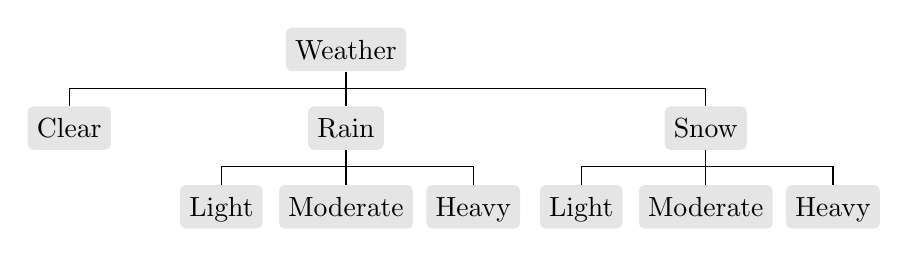
\begin{tikzpicture}
	% Place the nodes
	\node[tag](weather){Weather};
	\node[tag, below of=weather](rain){Rain};
	\node[tag, left of=rain, node distance=10em](clear){Clear};
	\node[tag, right of=rain, node distance=13em](snow){Snow};
	\node[tag, below of=rain](mod rain){Moderate};
	\node[tag, left of=mod rain, node distance=4.5em](light rain){Light};
	\node[tag, right of=mod rain, node distance=4.6em](heavy rain){Heavy};
	\node[tag, below of=snow](mod snow){Moderate};
	\node[tag, left of=mod snow, node distance=4.5em](light snow){Light};
	\node[tag, right of=mod snow, node distance=4.6em](heavy snow){Heavy};
	
	% Place the lines
	\node[helper, below of=weather](weather helper){};
	\node[helper, below of=rain](rain helper){};
	\node[helper, below of=snow](snow helper){};
	\draw (weather) -- (rain);
	\draw (weather) -- (weather helper) -| (clear);
	\draw (weather) -- (weather helper) -| (snow);
	\draw (rain) -- (mod rain);
	\draw (rain) -- (rain helper) -| (light rain);
	\draw (rain) -- (rain helper) -| (heavy rain);
	\draw (snow) -- (mod snow);
	\draw (snow) -- (snow helper) -| (light snow);
	\draw (snow) -- (snow helper) -| (heavy snow);
\end{tikzpicture}%

		} \\
		\subfloat[Tags for target description.]{
			\definecolor{TNOlightgray}{RGB}{222,222,231}%
\tikzstyle{tag}=[font=\sffamily, text height=.8em, text depth=.1em, fill=TNOlightgray, rounded corners=0.2em]%
\tikzstyle{diffheighttag}=[node distance=2.5em]%
\tikzstyle{helper}=[coordinate, node distance=1.5em]%
\tikzstyle{helper2}=[coordinate, node distance=4.0em]%
\begin{tikzpicture}
	% Place the nodes
	\node[tag](target){\footnotesize Target in front};
	\node[coordinate, below of=target](below target){};
	\node[coordinate, left of=below target, node distance=3.4em](following){};
	\node[tag, diffheighttag, below of=following](following2){\footnotesize Vehicle following};
	\node[tag, left of=following, node distance=3.5em](free){\footnotesize No target};
	\node[tag, right of=below target, node distance=4.4em](appearing){\footnotesize Target appearing};
	\node[coordinate, right of=appearing, node distance=4.5em](disappearing){};
	\node[tag, diffheighttag, below of=disappearing](disappearing2){\footnotesize Target disappearing};
	\node[coordinate, below of=following2, node distance=2.8em](braking){};
	\node[tag, diffheighttag, below of=braking](braking2){\footnotesize Braking};
	\node[tag, left of=braking2, node distance=3.7em](cruising){\footnotesize Cruising};
	\node[tag, right of=braking2, node distance=4.4em](accelerating){\footnotesize Accelerating};
	\node[coordinate, below of=appearing](below appearing){};
	\node[coordinate, diffheighttag, below of=below appearing](below appearing2){};
	\node[tag, left of=below appearing2, node distance=2.6em](cutin){\footnotesize Cut-in};
	\node[tag, right of=below appearing2, node distance=1.5em](gapclosing){\footnotesize Gap-closing};
	\node[coordinate, below of=disappearing2](below disappearing){};
	\node[coordinate, diffheighttag, below of=below disappearing](below disappearing2){};
	\node[tag, left of=below disappearing2, node distance=2.3em](cutout){\footnotesize Cut-out};
	\node[tag, right of=below disappearing2, node distance=2.3em](gapmaking){\footnotesize Gap-making};
	
	% Place the lines
	\node[helper, below of=target](target helper){};
	\node[helper2, below of=following2](following helper){};
	\node[helper2, below of=appearing](appearing helper){};
	\node[helper2, below of=disappearing2](disappearing helper){};
	\draw (target) -- (target helper) -| (free);
	\draw (target) -- (target helper) -| (following2);
	\draw (target) -- (target helper) -| (appearing);
	\draw (target) -- (target helper) -| (disappearing2);
	\draw (following2) -- (following helper) -| (cruising);
	\draw (following2) -- (braking2);
	\draw (following2) -- (following helper) -| (accelerating);
	\draw (appearing) -- (appearing helper) -| (cutin);
	\draw (appearing) -- (appearing helper) -| (gapclosing);
	\draw (disappearing2) -- (disappearing helper) -| (cutout);
	\draw (disappearing2) -- (disappearing helper) -| (gapmaking);
\end{tikzpicture}%

		}\\
		\subfloat[Tags for type of road, inspired from \cite{Bonnin2014}.]{
			\definecolor{TNOlightgray}{RGB}{222,222,231}%
\tikzstyle{tag}=[font=\sffamily, text height=.8em, text depth=.1em, fill=TNOlightgray, rounded corners=0.2em]%
\tikzstyle{helper}=[coordinate, node distance=1.4em]%
\tikzstyle{emph}=[fill=TNOred]
\begin{tikzpicture}
	% Place the nodes
	\node[tag, emph](road){Type of road};
	\node[coordinate, below of=road](below road){};
	\node[tag, left of=below road, node distance=10em, emph](highway){Highway};
	\node[tag, right of=below road, node distance=9.5em](inner city){Inner city};
	\node[tag, right of=inner city, node distance=10.5 em](remaining a){...};
	\node[coordinate, below of=highway](below highway){};
	\node[tag, left of=below highway, node distance=2em](exit){Exit};
	\node[tag, left of=exit, node distance=4em](entrance){Entrance};
	\node[tag, right of=below highway, node distance=2em, emph](merging highway){Merging};
	\node[tag, right of=merging highway, node distance=3.4em](remaining b){...};
	\node[tag, below of=inner city](intersection){Intersection};
	\node[tag, left of=intersection, node distance=8em](pedestrian crossing){Pedestrian crossing};
	\node[tag, right of=intersection, node distance=5.6em](merging inner city){Merging};
	\node[tag, right of=merging inner city, node distance=3.5em](remaining c){...};
	
	% Place the lines
	\node[helper, below of=road](road helper){};
	\node[helper, below of=highway](highway helper){};
	\node[helper, below of=inner city](inner city helper){};
	\draw (road) -- (road helper) -| (highway);
	\draw (road) -- (road helper) -| (inner city);
	\draw (road) -- (road helper) -| (remaining a);
	\draw (highway) -- (highway helper) -| (entrance);
	\draw (highway) -- (highway helper) -| (exit);
	\draw (highway) -- (highway helper) -| (merging highway);
	\draw (highway) -- (highway helper) -| (remaining b);
	\draw (inner city) -- (inner city helper) -| (pedestrian crossing);
	\draw (inner city) -- (intersection);
	\draw (inner city) -- (inner city helper) -| (merging inner city);
	\draw (inner city) -- (inner city helper) -| (remaining c);
\end{tikzpicture}%

		} \\
		\subfloat[Tags for the criticality, see \cite{ebner2011identifying}.]{
			\input{figures/tree_criticality.tikz}
		}
		\caption{Examples of tree structures with \emph{tags} for a scenario.}
		\label{fig:tag trees}
	\end{center}
\end{figure}

\subsection{Definition of events}
\label{sec:events}
% Introduction of this section
A scenario, for which the definition is proposed in Section~\ref{sec:scenario definition}, consists of events. Events can be seen as the `building blocks' of a scenario. The notion of event is extensively used in literature. In this section, a selected number of descriptions is presented. Next, a definition of event is given such that it suits our context.

% Literature review
The term event is used in many different fields, e.g.:
\begin{itemize}
	\item In computing, an event is an action or occurrence recognized by software. A common source of events are its users. An event may trigger a state transition \cite{breu1997towards}.
	\item Jeagwon Kim, a philosopher, writes: ``The term event ordinarily implies change'' \cite{kim1993supervenience}. Kim states that an event is composed of three elements: Objects, a property and a time or a temporal interval. 
	\item In probability theory, an event is an outcome or a set of outcomes of an experiment \cite{pfeiffer2013concepts}. For example, a thrown coin landing on its tail is an event.
	\item ``In relativity, an event is any occurrence with which a definite time and a definite location are associated; it is an idealization in the sense that any actual event is bound to have a finite extent both in time and in space'' \cite{sartori1996understanding}.
	\item In the field of hybrid theory, ``the continuous and discrete dynamics interact at `event' or `trigger' times when the continuous state hits certain prescribed sets in the continuous state space'' \cite{branicky1998hybridcontrol}. ``A hybrid system can be in one of several modes of operation, [...], and the system switches from one mode to another due to the occurrence of events.'' \cite{boel1999hybridcontrol}.
	\item In event-based control, a control action is computed when an event is triggered, as opposed to the more traditional approach where a control action is periodically computed \cite{heemels2012eventcontrol}. 
\end{itemize}

Before providing the definition of an event, the following is concluded about an event:

% It is a time instant
\subsubsection{An event corresponds to a time instant}
Whether it is regarding computing \cite{breu1997towards}, philosophy \cite{kim1993supervenience}, relativity \cite{sartori1996understanding}, hybrid or event-based control \cite{branicky1998hybridcontrol, boel1999hybridcontrol, heemels2012eventcontrol}, an event is happening at a time instant.

% Event should mark transition of a state from one set to another - mention relation with hybrid control
\subsubsection{An event marks the transition of a state}
During a traffic scenario, the states (see Section~\ref{sec:state} for a description of state) are continuously evolving. For example, when a vehicle moves from $A$ to $B$, the position changes. For the assessment methodology, it is required to parametrize the way the state evolves over time (e.g., see \cite{deGelder2017assessment}). Therefore, specific models will be employed to describe this (see Section~\ref{sec:model} for a description of model). These models, each with a fixed number of parameters, will only be valid for a certain time interval. Therefore, events should mark the transition from one model that is describing the state to another model describing the state.

%\subsubsection{An event marks (a cause of) a mode transition}
%Events mark the transition of mode, which is either a change of input, parameter or state. This is analogous to the way event is described in hybrid control \cite{boel1999hybridcontrol}.

% Give definition
Hence, we define an event as follows.
\begin{definition}[Event] \label{def:event}
	An event marks the time instant at which a transition of a state occurs, such that before and after an event, the state is described by a different model. %Furthermore, it marks the start and end of a time interval that can be qualitatively described.
\end{definition}

% Compare definition with literature and other remarks
% - Mention that it is basically similar to the definition adopted with hybrid control theory
% - Mention that before and after, different qualitative description
Definition~\ref{def:event} is in some way analogous to an event described in hybrid control \cite{boel1999hybridcontrol}. Here, an event describes the transition from one mode of operation to another mode of operation. In our application, i.e. events in traffic scenarios, ``mode of operation'' is described by a certain model with parameters assigned to it.

During the time interval between two events, or, in short, the inter-event time interval, a state is quantitatively described by a model. It is, however, possible to describe the way the state evolves during the inter-event time interval, i.e., the activity, in a qualitative manner. For example, when the longitudinal acceleration is negative during such an inter-event time interval, the activity can be described by the word `braking'. Another example is when at the event, the head lights are turned on. In that case, the activities before and after the event can be described as `lights off' and `lights on', respectively.

